%%%%%%%%%%%%%%%%%%%%%%%%%%%%%%%%%%%%%%%%%%%%%%%%%%%%%%%%%%%%%%%%%%%%%%%%%%%
% Chapter: Introduction
%%%%%%%%%%%%%%%%%%%%%%%%%%%%%%%%%%%%%%%%%%%%%%%%%%%%%%%%%%%%%%%%%%%%%%%%%%%
\nsl{Most computers are not on a desk. They are built into washing machines,
cars, heating systems, medical devices and smartphones, and they control
these devices without the user ever noticing that a computer is involved.
Such embedded systems have their own requirements. They must react in time,
work for years without a reset, run on a battery, cost a few euros at most,
and they must never endanger anybody.
\newline
This lecture covers the whole path from the requirements to a working
device. It starts with models and cyber-physical systems, continues with
processors and their programming in assembly, C, Rust and MicroPython, then
treats the peripherals and interfaces of a microcontroller, networking and
real-time operating systems. All examples run in the browser-based simulator
Wokwi or on Replit, so they can be tried without any hardware.
\newpage}

%==============================================================================
\section{What is an Embedded System?}
%==============================================================================
\begin{description}
\item[{\rot\bf Definition}]~\\
\defn{def:embedded system intro}
{An \textbf{embedded system} is a computer system that is part of a larger technical system and performs dedicated functions in it -- usually with requirements on timing, energy, reliability and cost.}
\bi
	\ite the user sees the device (a car, a coffee machine), not the computer in it
	\ite interaction with the environment through \textbf{sensors} and \textbf{actuators}, often without a screen or keyboard
	\ite the software is fixed for the purpose (``firmware''), updates are rare and must be safe
\ei
\os{\newpage}

\item[{\rot\bf Embedded systems are everywhere}]~\\[-3ex]
\bi
	\ite tens of billions of microcontrollers are produced every year -- many times more than PC and server processors
	\ite a modern car contains 70 to over 100 control units (engine, brakes, airbag, lights, seats, infotainment)
	\ite household: washing machine, heating, smart meter, router, TV, smart speaker
	\ite industry: programmable logic controllers, robots, drives, sensors with network interfaces
	\ite medicine: pacemakers, insulin pumps, ventilators
	\ite communication: smartphones (several processors), base stations, satellites
\ei
\os{\newpage}

\item[{\rot\bf Structure of an embedded system}]~\\[-3ex]
\begin{figure}[!hbtp]
     \begin{center}
	  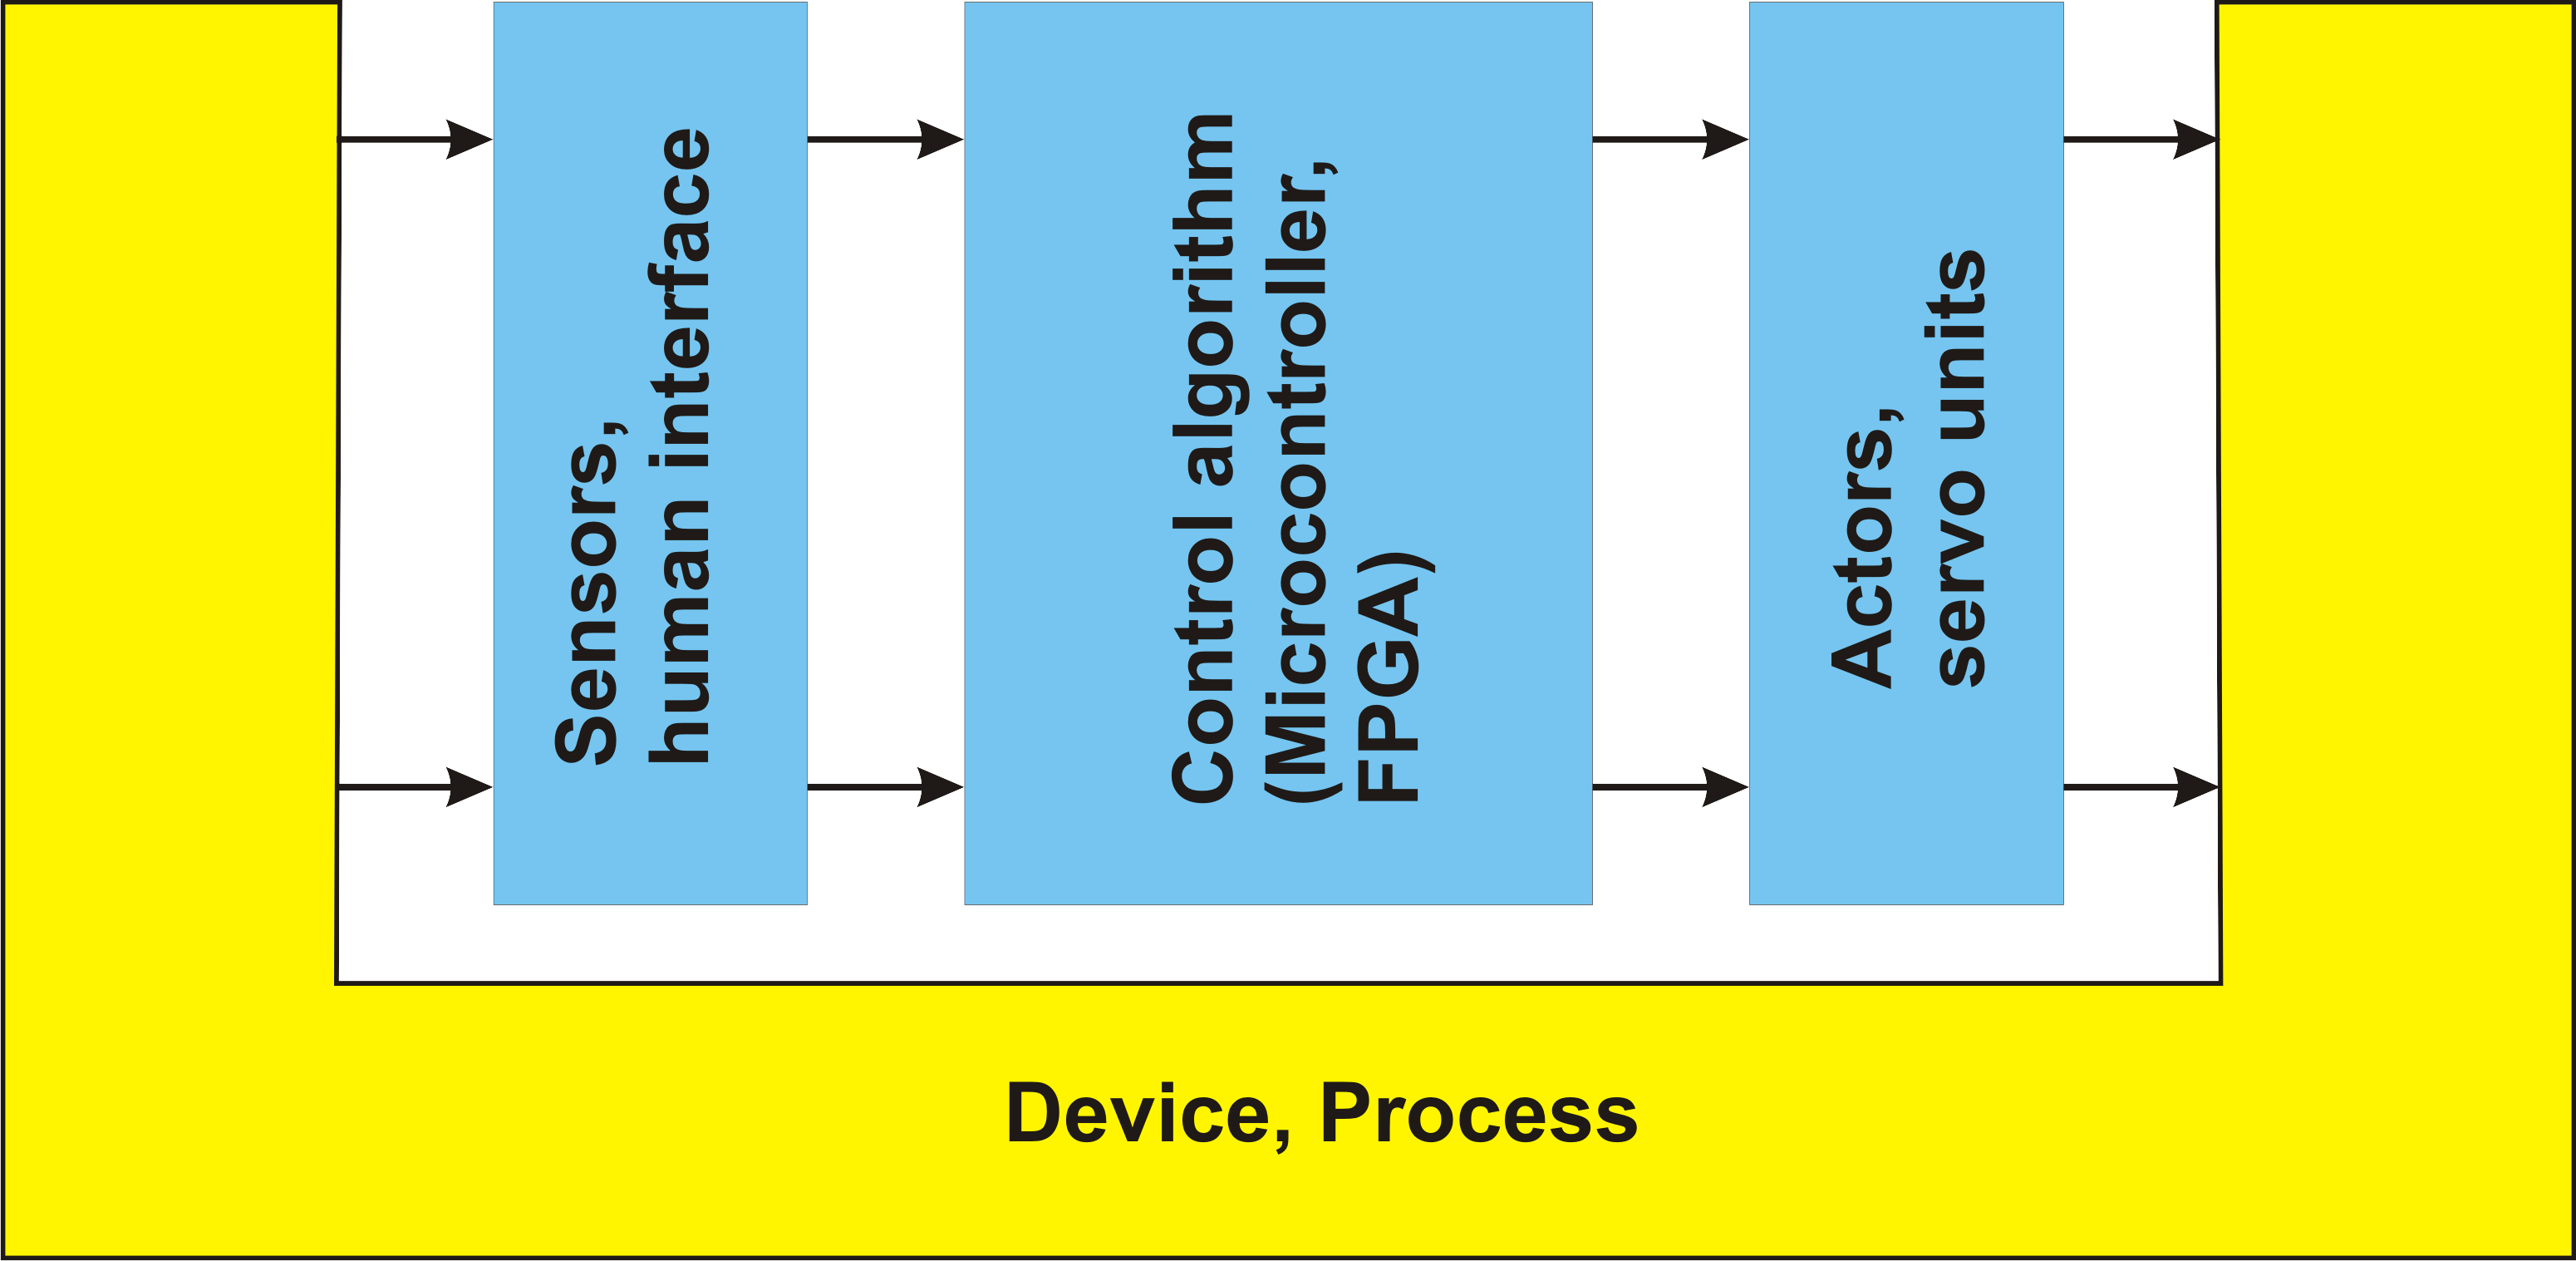
\epsfig{file=figures/Fig_1_10_Blockdiagram_Embedded_System,width=0.75\textwidth}\\
	  \caption{Block diagram of an embedded system}
     \end{center}
\end{figure}
\os{\newpage}

\begin{figure}[!hbtp]
     \begin{center}
	  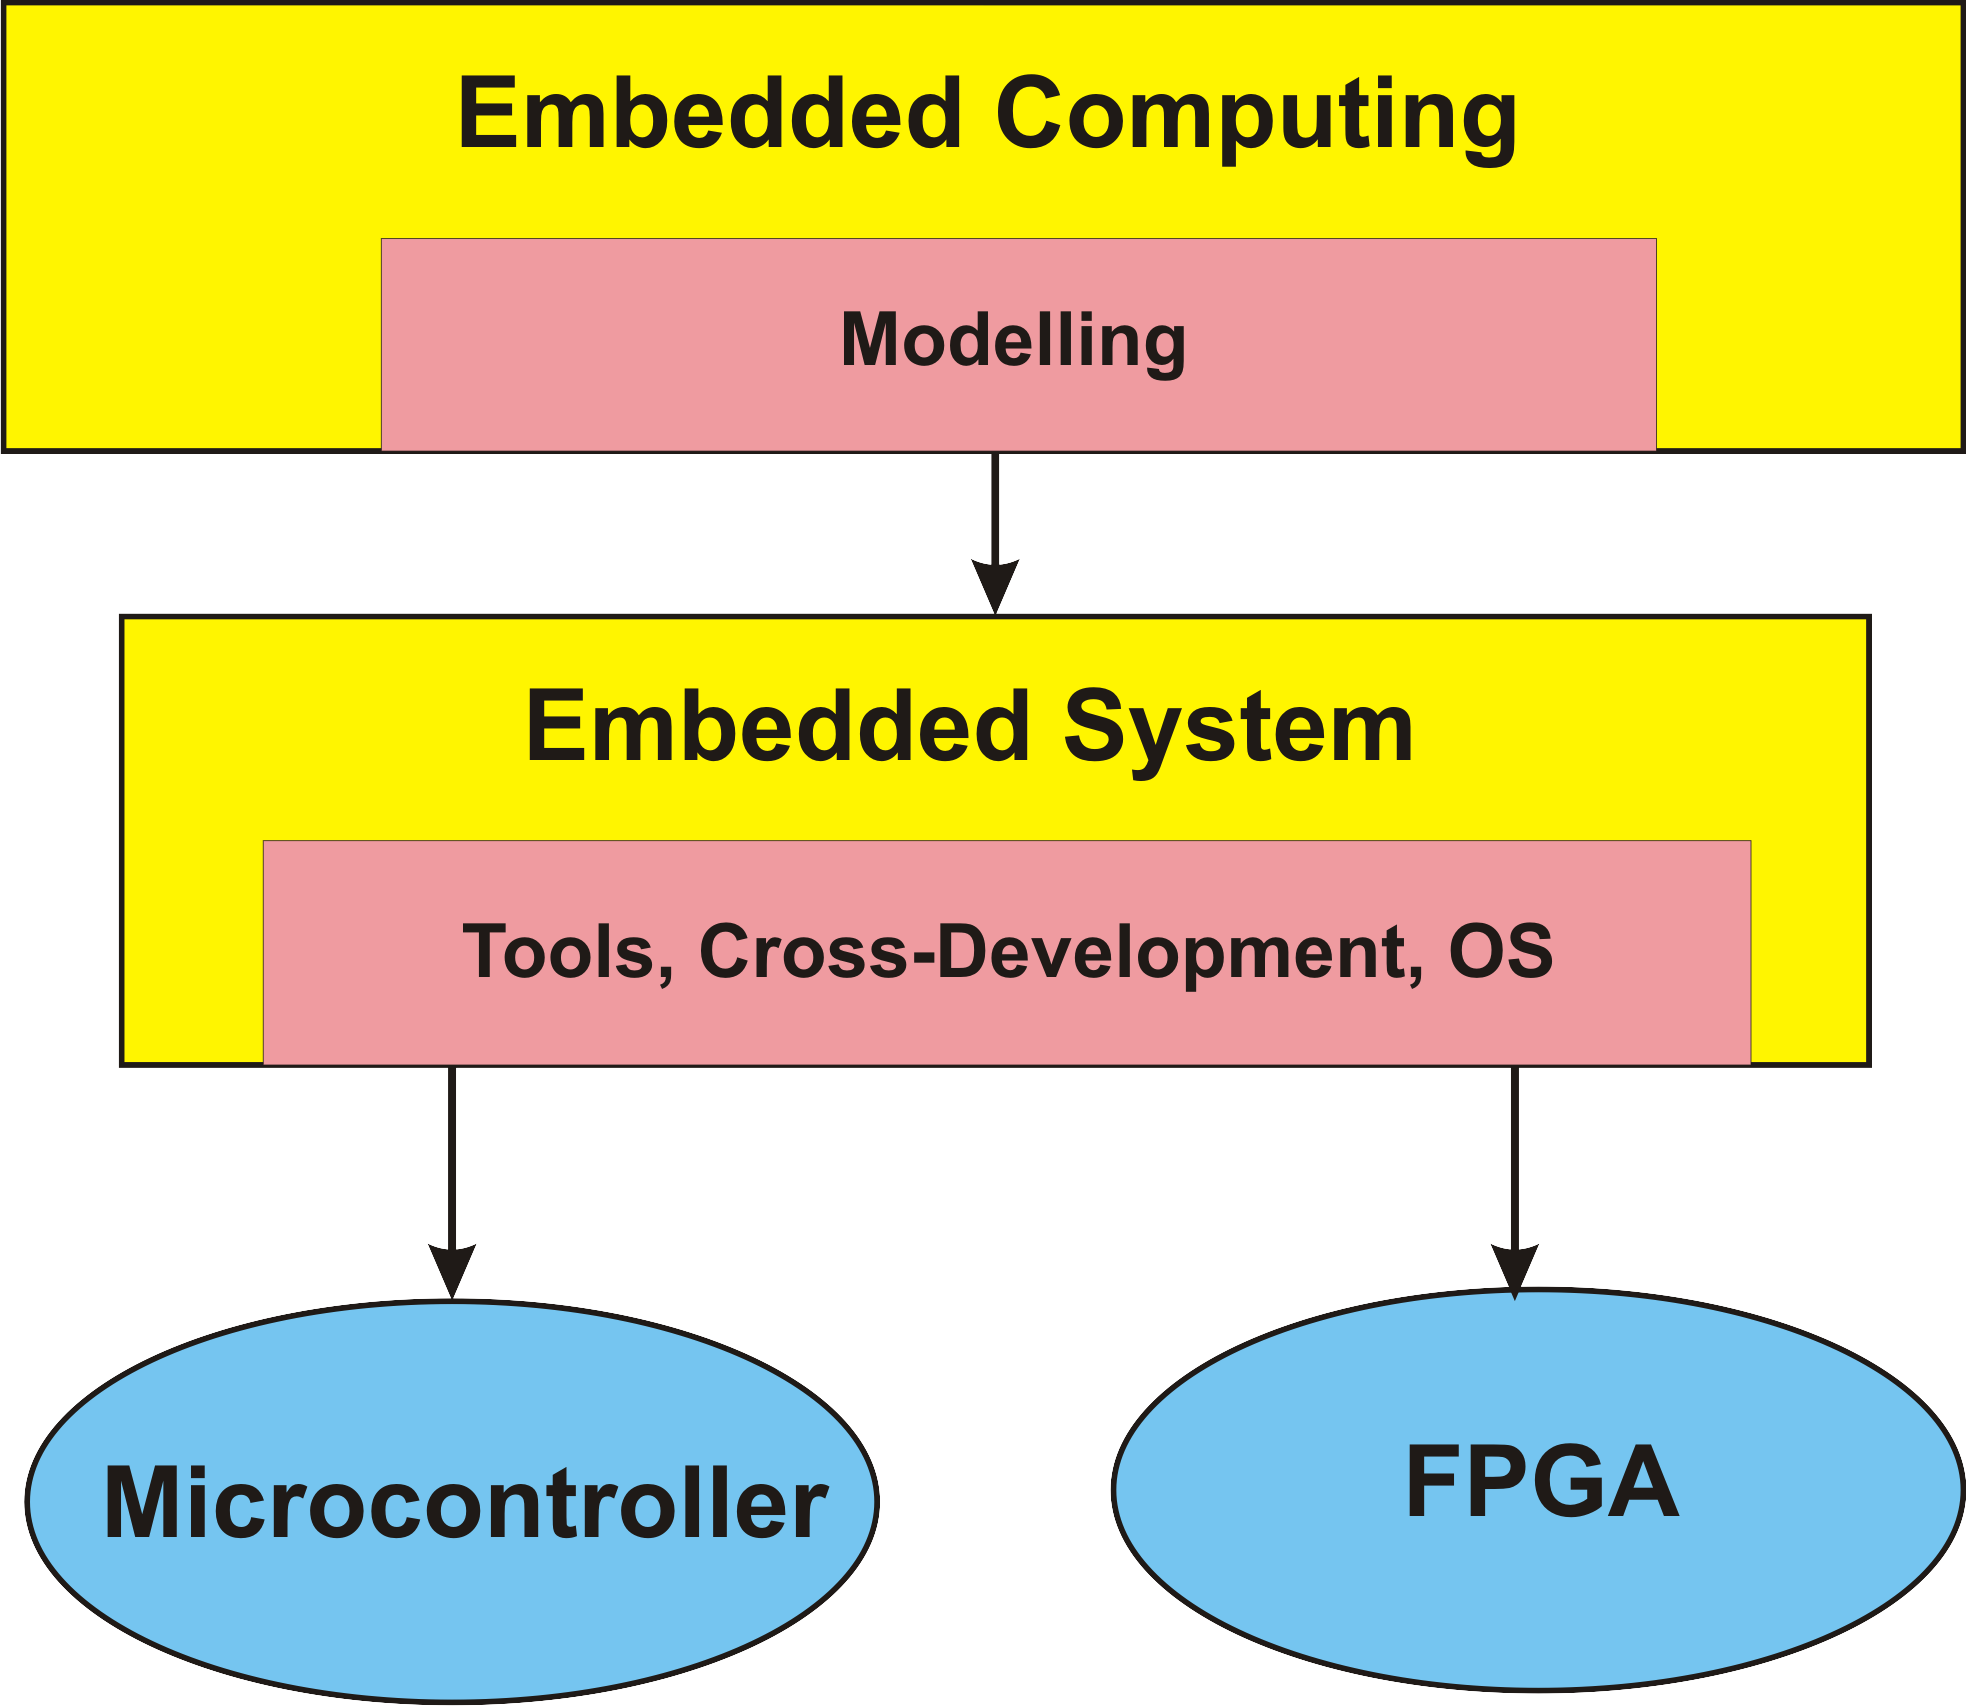
\epsfig{file=figures/Fig_1_9_Blockdiagram_Embedded_Computing,width=0.7\textwidth}\\
	  \caption{Embedded computing and the embedded system around it}
     \end{center}
\end{figure}
\os{\newpage}
\end{description}

%==============================================================================
\section{Historical Background}
%==============================================================================
\begin{description}
\item[{\rot\bf From room-sized computers to the microcontroller}]~\\[-3ex]
\begin{figure}[!hbtp]
\begin{center}
\resizebox{\textwidth}{!}{%
\begin{tikzpicture}[font=\sffamily\scriptsize,>=Stealth]
	\draw[->,thick] (0,0) -- (17.5,0);
	\foreach \x/\y/\t/\up in {
		0.3/1941/Zuse Z3: first programmable computer/1,
		1.4/1944/Harvard Mark I/0,
		2.6/1966/Apollo Guidance Computer/1,
		3.8/1971/Intel 4004: first microprocessor/0,
		5.0/1974/TMS1000: first microcontroller/1,
		6.2/1980/Intel 8051/0,
		7.4/1996/Atmel AVR/1,
		8.6/2004/ARM Cortex-M3/0,
		9.8/2005/Arduino/1,
		11.0/2010/RISC-V starts/0,
		12.2/2012/Raspberry Pi/1,
		13.4/2016/ESP32: Wi-Fi MCU/0,
		14.6/2021/RP2040/1,
		15.8/2024/RP2350: ARM or RISC-V/0} {
		\fill (\x,0) circle (2pt);
		\ifnum\up=1
			\draw (\x,0) -- (\x,0.6); \node[above,align=center,text width=16mm] at (\x,0.6) {\textbf{\y}\\\t};
		\else
			\draw (\x,0) -- (\x,-0.6); \node[below,align=center,text width=16mm] at (\x,-0.6) {\textbf{\y}\\\t};
		\fi
	}
\end{tikzpicture}}
\caption{Milestones on the way to today's embedded systems}
\end{center}
\end{figure}
\bi
	\ite the first computers (Zuse Z3 1941, Mark I 1944) filled rooms; the Apollo Guidance Computer (1966) was one of the first computers built into a vehicle
	\ite the microprocessor (1971) and the microcontroller with memory and I/O on one chip (1974) made embedded systems cheap
	\ite today a 32 bit microcontroller with Wi-Fi costs about one euro
\ei
\os{\newpage}

\item[{\rot\bf Computer generations}]~\\[-3ex]
\begin{center}
\resizebox{0.95\textwidth}{!}{%
\begin{tabular}{|c|c|c|c|}
\hline
\textbf{generation} & \textbf{period} & \textbf{technology} & \textbf{typical systems}\\
\hline
1 & 1945 -- 1955 & vacuum tubes & mainframes \\
2 & 1955 -- 1965 & transistors & mainframes, process control \\
3 & 1965 -- 1975 & integrated circuits & minicomputers \\
4 & 1975 -- & LSI / VLSI, microprocessors & workstations, PCs, microcontrollers \\
today & & systems on chip, many cores & smartphones, IoT, AI accelerators \\
\hline
\end{tabular}}
\end{center}
\bi
	\ite the trend continues: more functions on one chip, less energy per operation, lower price
	\ite \textbf{central vs.\ distributed}: instead of one central computer, many small connected controllers close to the sensors and actuators
\ei
\os{\newpage}
\end{description}

%==============================================================================
\section{Characteristics of Embedded Systems}
%==============================================================================
\begin{description}
\item[{\rot\bf Dependability}]~\\[-3ex]
\bi
	\ite \textbf{reliability}: probability that the system works correctly for a given time, provided it worked at the start
	\bi
		\ite operation for years without restart; recovery from errors by itself (watchdog)
	\ei
	\ite \textbf{maintainability}: how quickly the system works again after an error
	\ite \textbf{availability}: probability that the system works at a given time
	\ite \textbf{safety}: the system does not endanger people or the environment -- even if it fails
	\ite \textbf{security}: the system resists attacks; connected devices must be protected and updatable
\ei
\qbox{Even perfectly designed systems can fail if the assumptions about the workload and possible errors turn out to be wrong.
\newline
Dependability must be considered from the very beginning -- it cannot be added afterwards.}
\os{\newpage}

\item[{\rot\bf Efficiency}]~\\[-3ex]
\bi
	\ite \textbf{energy}: battery operation for months or years, sleep modes, energy harvesting
	\ite \textbf{code size and memory}: kilobytes instead of gigabytes; no hard disk
	\ite \textbf{run time}: real-time requirements -- a correct answer that arrives too late is wrong
	\ite \textbf{size and weight}: the electronics must fit into the device
	\ite \textbf{cost}: in a series of millions every cent counts; the development costs are spread over the number of devices
\ei
\os{\newpage}

\item[{\rot\bf Further characteristics}]~\\[-3ex]
\bi
	\ite \textbf{reactive}: continuous interaction with the environment, at its pace (chapter Modelling)
	\ite \textbf{real time}: deadlines are part of the specification (chapter Operating Systems)
	\ite \textbf{dedicated}: one purpose, known in advance -- hardware and software can be optimised for it
	\ite \textbf{heterogeneous}: hardware and software, analog and digital, different processors and networks in one system
	\ite \textbf{long lifetime}: industrial devices and cars are used for 10 to 20 years -- software must be maintained that long
	\ite \textbf{cyber-physical}: computation and physics are coupled in feedback loops (chapter Cyber-Physical Systems)
\ei
\os{\newpage}
\end{description}

%==============================================================================
\section{About this Lecture}
%==============================================================================
\begin{description}
\item[{\rot\bf Contents}]~\\[-3ex]
\begin{center}
\resizebox{0.95\textwidth}{!}{%
\begin{tabular}{|c|l|l|}
\hline
\textbf{chapter} & \textbf{topic} & \textbf{platform of the examples} \\
\hline
2 & Modelling: state machines, data flow & Pico (coffee machine FSM) \\
3 & Cyber-physical systems, Modelica & OpenModelica, Python \\
4 & Processors: AVR, Cortex-M, RISC-V & compiler output for 4 processors \\
5 & Programming: build process, assembly, C, Rust, MicroPython, debugging & Pico, PC \\
6 & Peripherals and interfaces: GPIO, interrupts, timers, ADC, UART, I$^2$C, SPI & Pico \\
7 & Networking: Wi-Fi, IP, TCP/UDP, sockets, HTTP, MQTT & ESP32-C3, PC \\
8 & Operating systems: FreeRTOS, Embassy, embedded Linux & ESP32-C3 \\
\hline
\end{tabular}}
\end{center}
\bi
	\ite every example exists in \textbf{C} and in \textbf{Rust} (some also in Python); all are in the folder \texttt{examples/} of the lecture repository
\ei
\os{\newpage}

\item[{\rot\bf Tools}]~\\[-3ex]
\bi
	\ite \textbf{Wokwi} (\url{https://wokwi.com}): simulator for Raspberry Pi Pico, ESP32, Arduino and STM32 in the browser -- with LEDs, buttons, sensors, displays, logic analyzer and Wi-Fi
	\bi
		\ite C (Arduino core + SDK) and MicroPython run directly in the browser
		\ite Rust: build locally with \texttt{cargo}, simulate with the Wokwi extension for VS Code
	\ei
	\ite \textbf{Replit} (\url{https://replit.com}) or your own PC: programs for the PC side (sockets, Python, Rust tests)
	\ite \textbf{Rust}: \texttt{rustup}, \texttt{cargo}, targets \texttt{thumbv6m-none-eabi} (Pico) and \texttt{riscv32imc-unknown-none-elf} (ESP32-C3)
	\ite \textbf{git}: all sources of the lecture and the examples are under version control
	\ite real hardware is optional: Raspberry Pi Pico and ESP32-C3 boards cost a few euros, and the same programs run on them
\ei
\os{\newpage}

\item[{\rot\bf Exercises}]~\\[-3ex]
\bi
	\ite List ten embedded systems in your home. For each: which sensors, which actuators, which communication?
	\ite Which of the characteristics (dependability, efficiency, real time, cost) is most important for an airbag control unit, a smart light bulb and a heart pacemaker?
	\ite Open \url{https://wokwi.com}, start a new Raspberry Pi Pico project and let the on-board LED blink.
\ei
\end{description}
